\subsubsection{Outlier Identification}
An important part of the analysis of the sound files is to identify when outliers arise. Our sponsor has expressed that being able to see when an outlier occurs and being able to listen to what caused it is important in drawing conclusions and finding interesting bits of information from a data set. Thus, two infographics seem reasonable, those being timelines and line charts. Both do relatively similar jobs, however a timeline is made specifically for information over time. The only upside to a line graph would be that each point on the graph would represent a sound file, and the results of its analysis. Being able to represent an output as a small dot on a chart and allowing the user to select or hover over that point to see which file caused the outlier is certainly desirable from a usability perspective. Implementing a full-fledged sound file analysis section seems a bit out of scope for this project, so a line graph used to represent each sound file in a data set and the results of each file\textquotesingle s analysis is the best way to help the user identify outliers in the data.\par

\begin{center}
  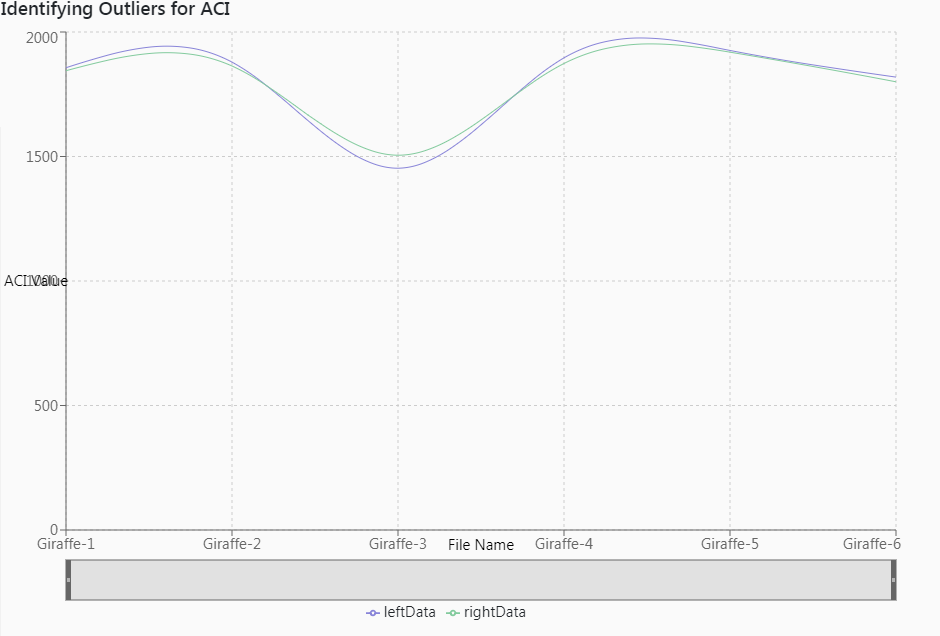
\includegraphics[width=\textwidth]{OutlierACIgraph1} \\[12pt]
  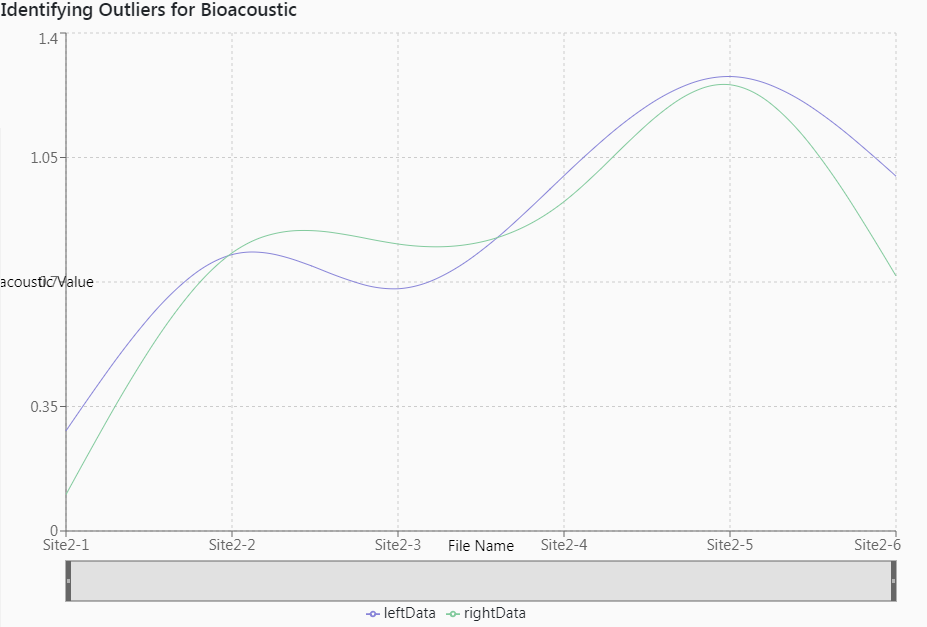
\includegraphics[width=\textwidth]{OutlierBAgraph1} \\[12pt]
\end{center}
The graphs above are for a data set comprised of files that the ACI and Bioacoustic Index was run on. The X axis displays the file name, while the Y axis labels the respective index value. Notice that file Giraffe 3 is much lower than the rest in the first graphic, and the file Site2-1 and Site2-5 also stand out in the second. Using these visuals, a researcher can quickly identify which files in their sets contain possibly interesting sounds to listen to in order to make further conclusions about their data.
